\documentclass{../industrial-development}
\graphicspath{{13-technical-support/}}

\title{Лекция №\,13 по теме «Организация~и~автоматизация технической поддержки программных продуктов»}
\author{ }
\date{}

\begin{document}

\begin{frame}
  \titlepage
\end{frame}

\begin{frame}{План лекции}
  \tableofcontents
\end{frame}  

%%%%%%%%%%%%%%%%%%%%%%%%%%%%%%%%%%%%%%%%%%страница 1
\section{Процесс сопровождения}
\subsection{Определение процесса сопровождения}


\begin{frame} \frametitle{Предпосылки к появлению традиционных методов}

	\begin{definition}
		\alert{Сопровождение программного обеспечения} 
		  - это процесс улучшения, оптимизации~и~устранения дефектов программного обеспечения (ПО) после передачи в~эксплуатацию
	\end{definition}
	
	Основная задача --- изменить~и~улучшить существующий программный продукт, сохраняя его целостность и~функциональную пригодность
	
\end{frame}

\lecturenotes
Процесс сопровождения является одной из фаз жизненного цикла программного обеспечения, следующей за передачей ПО в эксплуатацию, и завершается выводом его из эксплуатации. В ходе сопровождения в программу вносятся изменения, с тем, чтобы исправить обнаруженные в процессе использования дефекты и недоработки, для добавления новой функциональности, повышения удобства использования (юзабилити) и роста уровня использования ПО. По стандарту ISO/IEC 12207, этот процесс входит в 5 основных процессов жизненного цикла (ЖЦ) ПО: приобретение, поставка, разработка, эксплуатация, сопровождение. 
Этот процесс достаточно хорошо стандартизован. Упомянем только некоторые основные стандарты:
1)ISO/IEC 14764 (2006, русский перевод стандарта 1999 г. — 2002 г.);
2)ISO/IEC 12207 (2008, русский перевод стандарта 2010г.);
3)ISO 20000;
4)SWEBOK (2004 г.);
5)ITIL v3 (2007 г, обновление — 2011 г.);
6)COBIT v5 (2012 г.).


%%%%%%%%%%%%%%%%%%%%%%%%%%%%%%%%%%%%%%%%%%страница 2
\subsection{Задачи сопровождения}
\begin{frame} \frametitle{Задачи сопровождения}
	\begin{itemize}
		\item устранение сбоев, исправление ошибок
		\item улучшение дизайна 
		\item расширение функциональных возможностей 
		\item модернизация
		\item адаптация для возможности работы на другой аппаратной платформе
	\end{itemize}
\end{frame}

\lecturenotes

\begin{frame} \frametitle{Иерархия типов предложения по модификации ПО}
\centerline{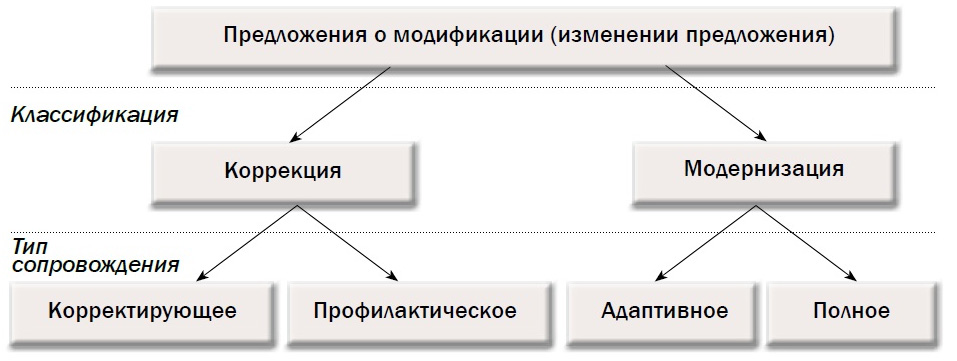
\includegraphics[width=\textwidth]{pic20.jpg}}
Иерархия типов предложения по модификации ПО (по стандарту ГОСТ Р ИСО/МЭК 14764-2002)
\end{frame}
\lecturenotes
Процесс сопровождения состоит из обработки заявок пользователей. Эти заявки целесообразно классифицировать по типам

%%%%%%%%%%%%%%%%%%%%%%%%%%%%%%%%%%%%%%%%%%страница 4
\subsection{Типы сопровождений}
\begin{frame} \frametitle{Типы сопровождений}
	\begin{definition}
		\alert{Корректирующее сопровождение} --- это реактивное изменение программного продукта для коррекции обнаруженных проблем (после обнаружения)
		\newline
		\newline
		\alert{Адаптивное сопровождение} --- изменение программного продукта после поставки для обеспечения его использования в условиях изменения его самого или окружающей среды
	\end{definition}
\end{frame}
\lecturenotes
Тип сопровождения — корректирующее — это реактивное изменение программного продукта для коррекции обнаруженных проблем (после обнаружения). Проблемы могут относиться к функциональности системы, ее интерфейсам, надежности и производительности работы.
Адаптивное сопровождение — изменение программного продукта после поставки для обеспечения его использования в условиях изменения его (программного продукта) или окружающей среды.


%%%%%%%%%%%%%%%%%%%%%%%%%%%%%%%%%%%%%%%%%%страница 5
\begin{frame} \frametitle{Типы сопровождений}
	\begin{definition}
		\alert{Полное (совершенствующее) сопровождение} --- это изменение программного продукта после поставки для улучшения производительности или удобства эксплуатации
		\newline
		\newline
		\alert{Профилактическое сопровождение} ---  это изменение программного продукта после поставки для выявления и исправления скрытых дефектов в ПО до того, как они станут явными ошибками
	\end{definition}
\end{frame}

\lecturenotes
Следует также отметить, что профилактическое и полное (совершенствующее) сопровождение относятся к проактивному подходу к сопровождению, при котором инициатива исходит от обслуживающего персонала, а корректирующее и адаптивное — к реактивному подходу, инициатива которого находится у пользователей.
Проактивному сопровождению необходимо уделять достаточно внимания, поскольку именно оно в наибольшей степени способствует повышению удовлетворенности пользователей и эффективному развитию программной системы

\begin{frame} \frametitle{Этапы процесса сопровождения}
\centerline{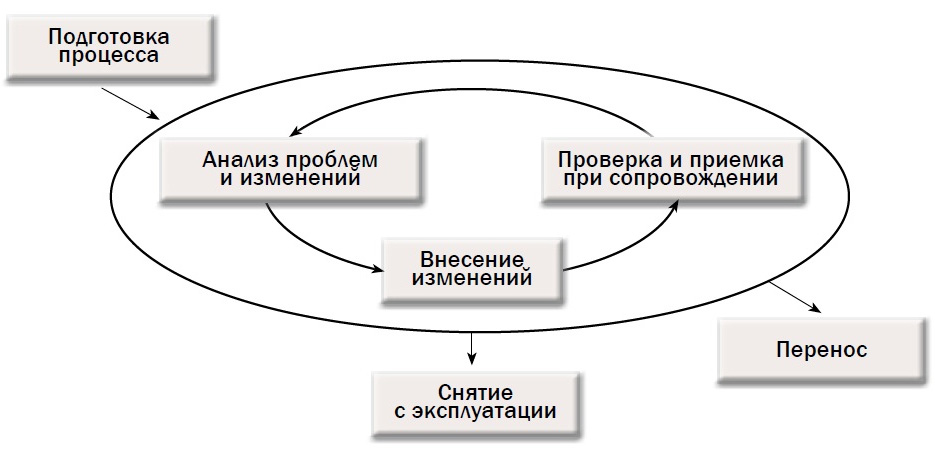
\includegraphics[width=\textwidth]{21.jpg}}
Общая структура процесса сопровождения (по стандарту ГОСТ Р ИСО/МЭК 14764-2002)
\end{frame}
\lecturenotes
Этапы процесса сопровождения основаны на цикле Деминга PDCA (Plan — Do — Check — Analyze) или «планируй — делай — проверяй — анализируй»

%%%%%%%%%%%%%%%%%%%%%%%%%%%%%%%%%%%%%%%%%%страница 6
\subsection{Концепция сопровождения}
\begin{frame} \frametitle{Концепция сопровождения}
Разделы документа о концепции сопровождения:
	\begin{enumerate}[1] \itemОбласти сопровождения программного средства
	\end{enumerate}
		\begin{itemize}
		\item Типы выполняемого сопровождения
		\item Сопровождаемый уровень документов
		\item Реакция (чувствительность) на сопровождение
		\item Обеспечиваемый уровень обучения персонала 
		\item Обеспечение поставки продукта
		\item Организация справочной службы («горячей линии») 
		\end{itemize}
\end{frame}
\lecturenotes
Формирование процесса сопровождения начинается с разработки концепции сопровождения. Такой документ, например, по стандарту ISO/IEC 14764 (Standard for Software Engineering — Software Maintenance), должен содержать следующие разделы:
1. Область сопровождения программного средства.
    1.1. Типы выполняемого сопровождения.
    1.2. Сопровождаемый уровень документов.
    1.3. Реакция (чувствительность) на сопровождение (определение ожиданий к сопровождению заказчика). 
    1.4. Обеспечиваемый уровень обучения персонала.
    1.5. Обеспечение поставки продукта.
    1.6. Организация справочной службы («горячей линии»).
2. Практическое применение (адаптация) данного процесса.
3. Определение организаций (лиц), ответственных за сопровождение.
4. Оценка стоимости сопровождения:
    4.1. Проезд до места расположения пользователя.
    4.2. Обучение как сопроводителей, так и пользователей.
    4.3. СПИ (среда программной инженерии) и СТПС (среда тестирования программного средства) и их ежегодное сопровождение.
    4.4. Персонал (зарплата и премии).

%%%%%%%%%%%%%%%%%%%%%%%%%%%%%%%%%%%%%%%%%%страница 7
\begin{frame} \frametitle{Концепции сопровождения}
	\begin{enumerate}[2]
	\item Практическое применение (адаптация) данного процесса
	\end{enumerate}
	\begin{enumerate}[3]
	\item Определение организаций (лиц), ответственных за сопровождение
	\end{enumerate}
	\begin{enumerate}[4]
	\item Оценка стоимости сопровождения: 
		\begin{itemize}
		\item Проезд до места расположения пользователя 
		\item Обучение как сопроводителей, так и пользователей
		\item СПИ (среда программной инженерии) и СТПС (среда тестирования программного средства) и их ежегодное сопровождение
		\item Персонал (зарплата и премии) 
		\end{itemize}
	\end{enumerate}
\end{frame}

\lecturenotes
Должен быть сформирован соответствующий план сопровождения. Этот план должен подготавливаться одновременно с разработкой программной системы. План должен определять, как пользователи будут размещать свои запросы на модификацию (изменения) или сообщать об ошибках, сбоях и проблемах.
Стандарт ГОСТ Р ИСО/МЭК 14764-2002 предлагает следующий состав такого плана:
a). Введение:
    описание сопровождаемой системы;
    определение исходных состояний программного средства;
    описание уровня требуемой поддержки;
    определение организаций, осуществляющих сопровождение;
    описание любых условий (протоколов), согласованных между заказчиком и поставщиками;
b). Концепция сопровождения (уже кратко описанная выше):
    описание концепции;
    описание уровня поддержки системы;
    установление периода поддержки;
    адаптация (практическое применение) процесса сопровождения;
c). Организационные работы и работы по сопровождению:
      1. роли и обязанности сопроводителя до поставки программного продукта:
            реализация процесса;
            определение инфраструктуры процесса;
            установление процесса обучения;
            установление процесса сопровождения;
     2. роли и обязанности сопроводителя после поставки программного продукта:
            реализация процесса;
            анализы проблем и модификаций (изменений);
            реализация (внесение) модификаций (изменений);
            рассмотрение и принятие модификаций (изменений);
            перенос программного средства в новую среду;
            снятие программного средства с эксплуатации;
            решение проблем (включая справочную службу);
            при необходимости — обучение персонала (сопроводителя и пользователя);
            усовершенствование процесса;
      3. роль пользователя:
        приемочные испытания;
        взаимосвязи (интерфейсы) с другими организациями;
d). Ресурсы:
      1. персонал:
        состав персонала для конкретного проекта; Структура, отвечающая за сопровождение, должна проводить общую деятельность по бизнес-планированию, касающуюся бюджетирования, финансового менеджмента и управления человеческими ресурсами в области сопровождения.
      2. программные средства:
        определение программных средств, необходимых для поддержки эксплуатации системы (с учетом системных требований и требований к СПИ, СТПС и инструментальным средствам);
      3. технические средства:
        определение технических средств, необходимых для поддержки эксплуатации системы (с учетом системных требований и требований к СПИ, СТПС и инструментальным средствам);
      4. оборудование (аппаратура):
        определение требований к оборудованию (аппаратуре) системы (помимо технических средств вычислительной техники);
      5. документы:
        план обеспечения качества;
        план управления проектом;
        план управления конфигурацией;
        документы разработки;
        руководства по сопровождению;
        план проведения верификации;
        план проведения аттестации (валидации);
        план тестирования, процедуры тестирования и отчеты о тестировании;
        план обучения;
        руководство (а) пользователя;
      6. данные;
      7. другие требования к ресурсам (при необходимости);
e). Процесс (как должна быть выполнена конкретная деятельность):
      1. процесс, выполняемый сопроводителем (приводят общее описание процесса без детализации в плане сопровождения всего процесса);
      2. процесс адаптации (практического применения сопровождения к условиям проекта);
f). Обучение:
      1. определение уровня обучения, необходимого для сопроводителя и пользователей;
g). Протоколы и отчеты по сопровождению:
      1. перечень запросов пользователя на оказание услуг по сопровождению, предложение о модификациях или отчеты о проблемах;
      2. состояния запросов (предложений, отчетов) по категориям;
      3. приоритеты запросов (предложений, отчетов);
      4. контрольные данные, собранные при работах по сопровождению.


%%%%%%%%%%%%%%%%%%%%%%%%%%%%%%%%%%%%%%%%%%страница 9
\begin{frame} \frametitle{Роли и обязанности сопроводителя ДО поставки программного продукта}
	\begin{itemize}
	\item Реализация процесса 
	\item Определение инфраструктуры процесса 
	\item Установление процесса обучения 
	\item Установление процесса сопровождения 
	\end{itemize}
\end{frame}

\lecturenotes

%%%%%%%%%%%%%%%%%%%%%%%%%%%%%%%%%%%%%%%%%%страница 10
\begin{frame} \frametitle{Роли и обязанности сопроводителя ПОСЛЕ поставки программного продукта}
	\begin{itemize}
		\item Реализация процесса
		\item Анализы проблем и модификаций (изменений)  
		\item Реализация (внесение) модификаций (изменений) 
		\item Рассмотрение и принятие модификаций (изменений) 
		\item Перенос программного средства в новую среду
	\end{itemize}
\end{frame}

\lecturenotes

%%%%%%%%%%%%%%%%%%%%%%%%%%%%%%%%%%%%%%%%%%страница 11
\begin{frame} \frametitle{Роли и обязанности сопроводителя ПОСЛЕ поставки программного продукта}
	\begin{itemize}
		\item Снятие программного средства с эксплуатации 
		\item Решение проблем (включая справочную службу) 
		\item При необходимости — обучение персонала (сопроводителя и пользователя) 
		\item Усовершенствование процесса
	\end{itemize}
	\item Роль пользователя:
	\begin{itemize}
		\item Приемочные испытания  
		\item Взаимосвязи (интерфейсы) с другими организациями
	\end{itemize}
\end{frame}

\lecturenotes


%%%%%%%%%%%%%%%%%%%%%%%%%%%%%%%%%%%%%%%%%%страница 12
\subsection{Ресурсы}
\begin{frame} \frametitle{Ресурсы}
	\begin{itemize} 
	    \item Персонал
		\item Программные средства 
		\item Технические средства
		\item Оборудование (аппаратура)
		\item Документы
		\item Данные
	\end{itemize}
\end{frame}

\lecturenotes
Структура, отвечающая за сопровождение, должна проводить общую деятельность по бизнес-планированию, касающуюся бюджетирования, финансового менеджмента и управления человеческими ресурсами в области сопровождения. 
1) состав персонала для конкретного проекта;
2)определение программных средств, необходимых для поддержки эксплуатации системы (с учетом системных требований и требований к СПИ, СТПС и инструментальным средствам); 
4)определение требований к оборудованию (аппаратуре) системы (помимо технических средств вычислительной техники); 

%%%%%%%%%%%%%%%%%%%%%%%%%%%%%%%%%%%%%%%%%%страница 13
\begin{frame} \frametitle{Ресурсы}
	Документы:
	\begin{itemize}
		\item План обеспечения качества
		\item План управления проектом 
		\item План управления конфигурацией 
		\item Документы разработки 
		\item Руководства по сопровождению 
		\item План проведения верификации 
		\item План тестирования, процедуры тестирования и~отчеты~о~тестировании 
		\item План обучения 
		\item Руководство пользователя
	\end{itemize}
	
\end{frame}

\lecturenotes



%%%%%%%%%%%%%%%%%%%%%%%%%%%%%%%%%%%%%%%%%%страница 22
\section{Техническая поддержка}

\subsection{Понятие технической поддержки}

\begin{frame} \frametitle{Техническая поддержка}
	\begin{definition} 
		\alert {Техническая поддержка} -- это сервисная структура, разрешающая проблемы пользователей с компьютерами, аппаратным и программным обеспечением
	\end{definition}
	Важная функциональная составляющая ITIL (библиотека инфраструктуры информационных технологий), позволяющая выявить проблемные участки инфраструктуры ИТ, оценить эффективность работы подразделения ИТ
\end{frame}
\lecturenotes

\subsection{Схема организации технической поддержки}
\begin{frame} \frametitle{Схема организации технической поддержки}
    \centerline{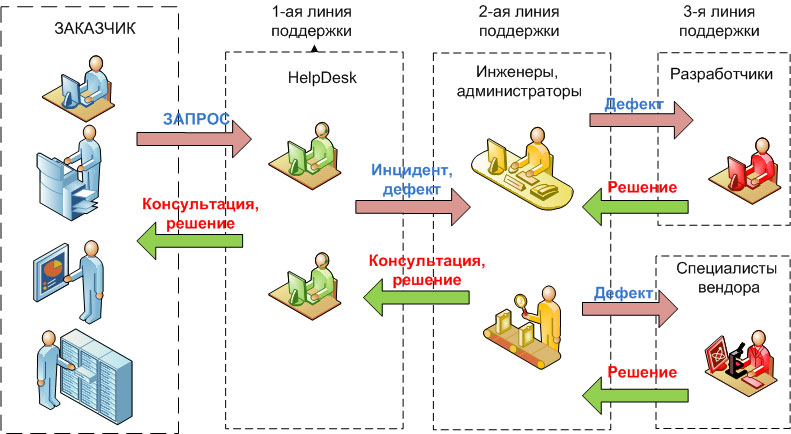
\includegraphics[width=\textwidth]{structure.jpg}}
\end{frame}

\lecturenotes

\begin{frame} \frametitle{Этап заказчика}

Техническая поддержка обычно предоставляется 
	\begin{itemize}
        \item по телефону
        \item по электронной почте
        \item с использованием специальных программ(helpdesk) (1С ИТИЛИУМ, eStreamDesk, Mojo, DIRECTUM, HP, IBM)
	\end{itemize}
\end{frame}

\lecturenotes

\begin{frame} \frametitle{Первая линия поддержки}

    Операторы (1-ая линия поддержки, Call-center) — регистрируют обращение, при возможности помогают пользователю самостоятельно, либо делегируют (передают и контролирует выполнение) заявку на вторую линию поддержки.
    \newline
    \newline
    Они, в отличие от остальных специалистов ИТ, ориентированы именно на общение с~простыми пользователями и призваны решать несложные (по уровню технической компетенции) обращения пользователей, а также реагировать на доступные их пониманию сообщения систем мониторинга

\end{frame}
\lecturenotes

\begin{frame} \frametitle{Вторая линия поддержки}

    Получает заявки от первой линии, работает по ним, при необходимости привлекая к~решению проблемы специалистов из смежных отделов (системные администраторы, поддержка POS-терминалов, поддержка специального ПО и~т.~д.)
    \newline
    \newline
    В обязанности специалистов второго уровня входят: 
	\begin{itemize}
        \item контакт и оказание помощи персоналу первой линии
        \item фиксация и последующий анализ инцидента
        \item решение проблемы
        \item передача данных по решенной проблеме на первый уровень
	\end{itemize}
\end{frame}
\lecturenotes
Специалисты второго уровня могут, например, пройти дополнительное обучение по поддержке распространенных операционных систем (например, Microsoft Windows) или аппаратных средств~и, следовательно, иметь возможность решать более сложные задачи, затрагивающие распространенные технологические решения.
Вторая линия поддержки — получает заявки от первой линии, работает по ним, при необходимости привлекая к~решению проблемы специалистов из смежных отделов (системные администраторы, поддержка POS-терминалов, поддержка специального ПО, поддержка специального оборудования (Дилинг) и~т.~д.). Помогает избавиться от случаев загруженности специалиста несложными, но объемными задачами.

\begin{frame} \frametitle{Третья линия поддержки}

    Обеспечивается как правило производителями оборудования и разработчиками системного программного обеспечения, а~также разработчиками специализированного прикладного программного обеспечения на основании договоров технического обслуживания и сопровождения программного обеспечения.
    \newline
    \newline
    Заявки на третью линию оформляются со второй линии в~случае если специалистам второй линии недостаточно компетенции для решения проблемы  

\end{frame}
\lecturenotes
В компаниях, которые разрабатывают собственное программное обеспечение, довольно распространена практика выделения групп поддержки уровня 3, отвечающих за конкретные приложения или службы


\begin{frame} \frametitle{Пример трехуровневой системы техподдержки}
    \begin{itemize}
        \item Уровень пользователя - приложение с формой обратной связи, телефонный номер, электронная почта
        \item 1-ая линия: диспетчер, отвечающий на звонки и обрабатывающий заявки
        \item 2-ая линия: администратор, решающий проблемы на компьютере пользователя средствами самого приложения
        \item 3-я линия: разработчик, напрямую обращающийся к базе и обновляющий приложение
    \end{itemize}
\end{frame}
\lecturenotes


\begin{frame} \frametitle{Пример обработки заявки} 
    \begin{enumerate}
        \item[1] Пользователь обнаруживает проблему, звонит диспетчеру
        \item[2] Диспетчер задаёт типовые вопросы (Какая версия программы используется?), проверяет корректность действий пользователя (На какую кнопочку вы нажимали? Какие данные вводили?), предлагает последовательность действий и проводит её вместе с пользователем. В большинстве случаев решает проблему, иначе передает заявку администратору
    \end{enumerate}
\end{frame}
\lecturenotes

\begin{frame} \frametitle{Пример обработки заявки} 
    \begin{enumerate}
        \item[3] Администратор удалённо подключается к компьютеру пользователя и сам пытается повторить ошибочный сценарий. Обновляет версию программы, исправляет конфигурацию. Если не удается выяснить причину проблемы или ошибка происходит непосредственно в самой программе, заявка передается разработчику
        \item[4] Разработчик находит причину ошибки в исходном коде или базе данных, вносит необходимые изменения. Выпускается новая версия приложения
    \end{enumerate}
\end{frame}
\lecturenotes

\begin{frame} \frametitle{Достоинства}
	\begin{itemize} 
		\item Заказчикам предоставлено «единое окно» для взаимодействия с ИТ-поддержкой, независимо от характера обращения
		\item Специалисты с общими техническими навыками, необходимыми для работы в поддержке уровня 1 и 2, легко доступны на рынке труда. Одновременно это упрощает вывод на аутсорсинг одного или обоих этих уровней, что также часто встречается
		\item Специализированные технические ресурсы могут быть ограждены от прямого контакта с пользователями. Это гарантирует, что заявки к ним попадают только после корректного анализа
	\end{itemize}
\end{frame}

\begin{frame} \frametitle{Недостатки}
	\begin{itemize} 
		\item Многоуровневая поддержка создает несколько очередей
		\item Лишние временные затраты: заявка проходит несколько уровней поддержки, на каждом из которых выполняются попытки её решения
		\item «Отфутболивание» задач: заявка может возвращаться на предыдущий уровень при неверной маршрутизации или для дополнительной информации
	\end{itemize}
\end{frame}

\lecturenotes Хотя поддержка первого уровня стремится быть реактивной и в реальном времени, любая заявка, которая не может быть решена на этом уровне, сразу же попадает в очередь. Её сущность меняется, превращаясь из текущей задачи в запись в бэклоге.



\subsection{Классификация}
\begin{frame} \frametitle{Классификация по типу оплаты}
	\begin{itemize} 
		\item {Время и материал}: этот тип поддержки распространен в технологической отрасли. Также известная как ИТ-поддержка <<break-fix>>, оплата материалов и плата за обслуживание технического персонала возлагается на клиента по заранее согласованной ставке
	\end{itemize}
\end{frame}

\begin{frame} \frametitle{Классификация по типу оплаты}
	\begin{itemize} 
        \item {Управляемые услуги}: обычно это предоставляется крупным клиентам, а не отдельным потребителям. Перечень четко определенных услуг и показателей эффективности предоставляется клиенту на постоянной основе по фиксированной ставке, которая согласовывается по контракту. Предоставляемые услуги могут быть круглосуточным мониторингом серверов, круглосуточной службой поддержки и т.~п. Это может включать посещения на месте, когда проблемы не могут быть решены удаленно
	\end{itemize}
\end{frame}

\begin{frame} \frametitle{Классификация по типу оплаты}
	\begin{itemize} 
        \item {Блокировка часов}: это предоплаченная система поддержки, в которой клиент платит определенное количество времени, которое может использоваться в~месяц или в год. Это позволяет клиентам гибко использовать часы без проблем с бумажной работой или несколькими счетами
	\end{itemize}
\end{frame}

\lecturenotes

\begin{frame} \frametitle{Основные функции систем автоматизации службы поддержки}
	\begin{itemize} 
		\item реализация полного жизненного цикла обработки заявок пользователя: регистрация, назначение и эскалация, закрытие
		\item предоставление web-доступа пользователям для самостоятельной регистрации заявок
		\item ведение Базы конфигурации, в которой хранится вся информация об элементах ИТ-инфраструктуры
		\item ведение Базы знаний
	\end{itemize}
\end{frame}
\lecturenotes

\begin{frame} \frametitle{Основные требования к системам автоматизации службы поддержки}
	\begin{itemize} 
		\item единая точка регистрации заявок пользователей, возможность регистрации заявок сотрудником службы технической поддержки от имени пользователя
		\item поддержка средств контроля сроков выполнения заявок на основании сервисных контрактов с потребителями ИТ-услуг, внутренних контрактов службы ИТ и контрактов с внешними поставщиками ИТ услуг
		\item ручные и автоматические назначения исполнителей
		\item поддержка вложенных процессов по механизму дерево/ветки
		\item делегирование заявки между линиями технической поддержки
		\item поддержка интеграции с внешними системами управления
	\end{itemize}
\end{frame}
\lecturenotes


\subsection{DIRECTUM}
\begin{frame} \frametitle{DIRECTUM}

    Helpdesk на базе системы DIRECTUM – автоматизация работы службы поддержки организации на базе системы электронного документооборота DIRECUM
    \newline
    \newline
    Helpdesk на базе DIRECTUM позволяет вести базу компьютерной техники в представлении системных блок, мониторов, принтеров с закреплением их за определенными сотрудниками организации и ведением истории изменений по ним, вплоть до утилизации соответствующей техники

\end{frame}
\lecturenotes

\begin{frame} \frametitle{Главное окно Help Desk}
\centerline{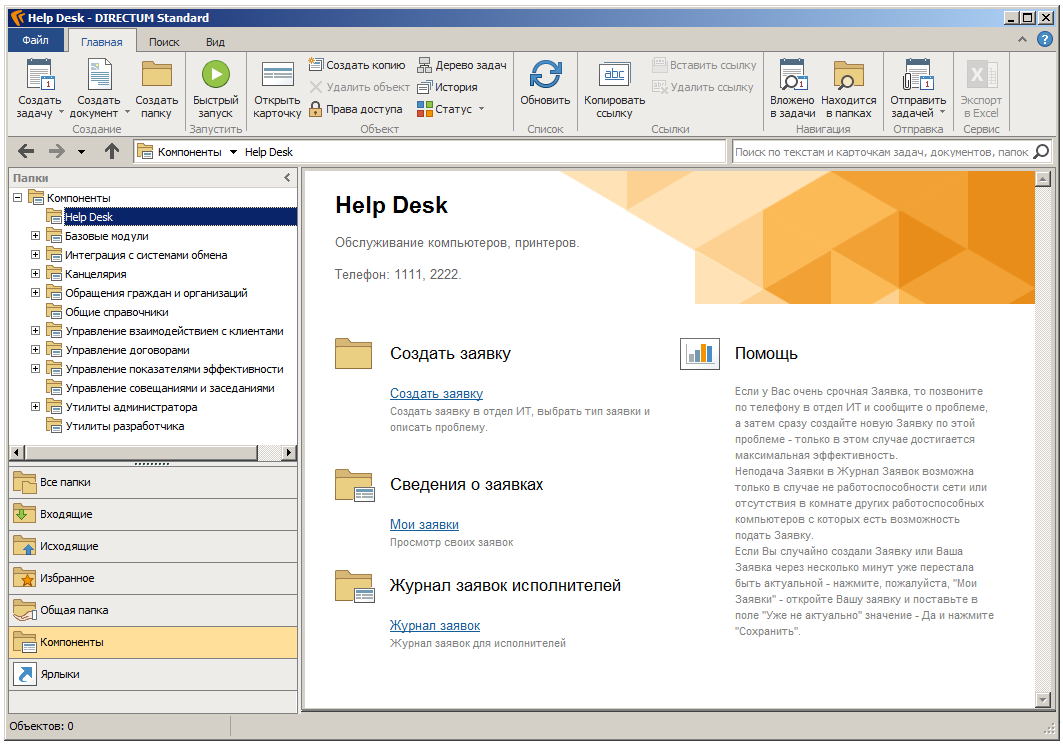
\includegraphics[width=\textwidth]{pic1.png}}
\end{frame}
\lecturenotes
Подача заявок сотрудниками осуществляется либо с помощью обложки в проводнике DIRECTUM либо с помощью внутреннего корпоративного сайта, на котором размещаются соответствующие ссылки на доступные действия

\begin{frame} \frametitle{Список текущих проблем}
\centerline{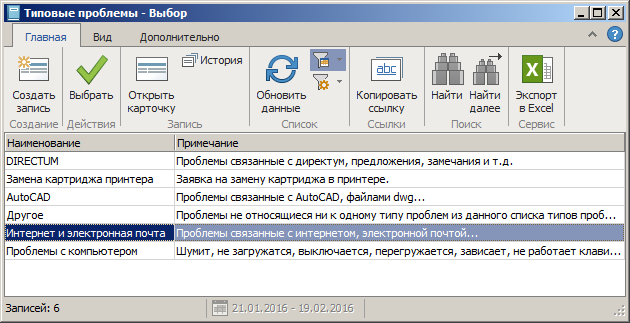
\includegraphics[width=\textwidth]{pic2.png}}
\end{frame}
\lecturenotes
При подаче заявки сотрудником организации сначала указывается тип проблемы из списка типовых проблем и в следующем окне задается краткое описание проблемы. 

\begin{frame} \frametitle{Просмотр описания проблемы}
\centerline{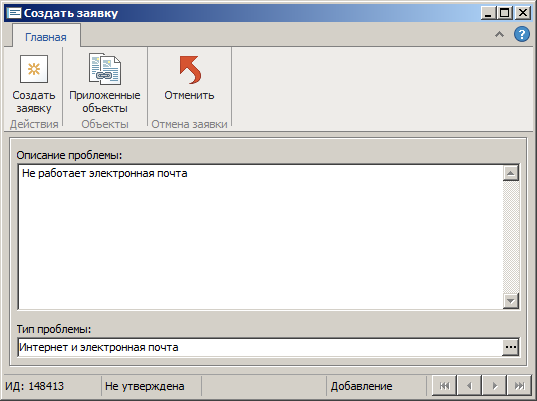
\includegraphics[height=7.5cm]{pic3.png}}
\end{frame}
\lecturenotes
При необходимости можно приложить ссылки к заявке на любые объекты системы DIRECTUM, например, документы или записи справочников. Таким образом, все заявки сотрудников группируются по типам проблем.

\begin{frame} \frametitle{Карточка заявки}
\centerline{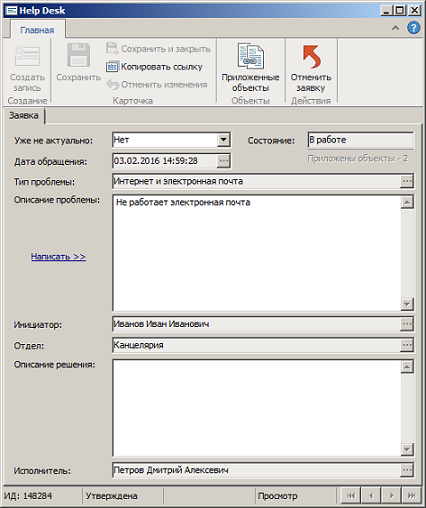
\includegraphics[height=7.5cm]{pic4.png}}
\end{frame}
\lecturenotes
Карточка заявки в представлении для сотрудников организации даёт возможность написать дополнительную информацию, приложить дополнительно объекты системы, отменить заявку, например, если она уже потеряла актуальность, посмотреть состояние заявки и ознакомится с описанием решения проблемы.

\begin{frame} \frametitle{Состояния заявок}
\centerline{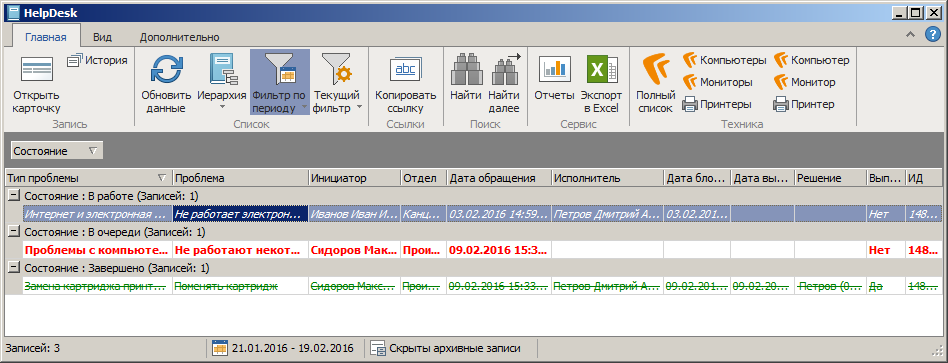
\includegraphics[width=\textwidth]{pic5.png}}
\end{frame}
\lecturenotes
Заявки имеют различные стили отображения в зависимости от своего состояния. Завершенные заявки помечаются как архивные записи с помощью стандартных средств DIRECTUM и не отображаются на экране, не нагружая систему, но их можно отобразить по необходимости.

\begin{frame} \frametitle{Состояния заявок}
	Доступны следующие состояния заявок:
	\begin{itemize}
		\item В очереди: назначается по умолчанию при создании заявки
		\item В работе: устанавливается при появлении назначении исполнителя
		\item Приостановлено: заявка отложена по какой-либо причине
		\item Завершено: заявка выполнена
		\item Отменено: заявка отменена по какой-либо причине
	\end{itemize}
\end{frame}
\lecturenotes

\begin{frame} \frametitle{Обработка заявки}
\centerline{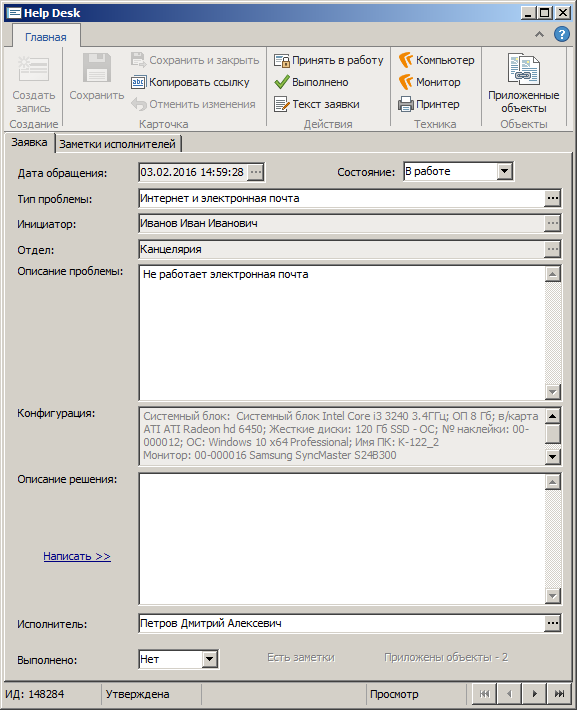
\includegraphics[height=7.5cm]{pic6.png}}
\end{frame}
\lecturenotes
Сотрудники службы поддержки осуществляют обработку заявок, поступающих от сотрудников организации и оперативно решают возникшие трудности, получив информацию в виде заявки с отображением информации о сотруднике с помощью всплывающих подсказок DIRECTUM и на основе информации о закреплённой за сотрудником техники.
При смене исполнителя или назначении нового исполнителя – новому исполнителю отправляется уведомление о том, что он назначен исполнителем у такой-то заявки. При завершении работ по заявке у исполнителя есть возможность отправить уведомление инициатору заявки о её выполнении.

\begin{frame} \frametitle{Информация по комплектующим}
\centerline{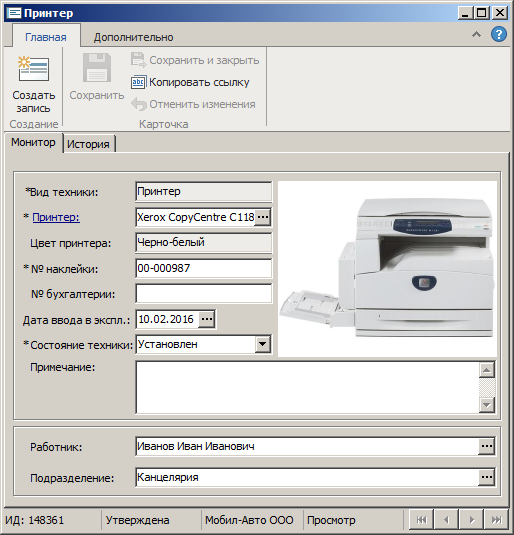
\includegraphics[height=7.5cm]{pic7.png}}
\end{frame}
\lecturenotes
В представлении исполнителя можно посмотреть детальную конфигурацию системного блока, историю изменений и кем были произведены изменения. Информация по основным комплектующим выбирается из соответствующих справочников, т.к. эта информация является статической и меняется очень редко, если что-то сломалось. Если в справочниках нет нужной модели оборудования, то она добавляется в справочник сотрудниками службы поддержки.

\begin{frame} \frametitle{Информация по комплектующим}
В представлении исполнителя можно посмотреть детальную конфигурацию системного блока, историю изменений и кем были произведены изменения. Информация по основным комплектующим выбирается из соответствующих справочников 
\newline
	Доступны следующие состояния техники:
	\begin{itemize}
		\item В резерве
		\item Установлен
		\item Не рабочий
		\item Утилизирован
	\end{itemize}
	
\end{frame}
\lecturenotes

\begin{frame} \frametitle{Список техники сотрудника}
\centerline{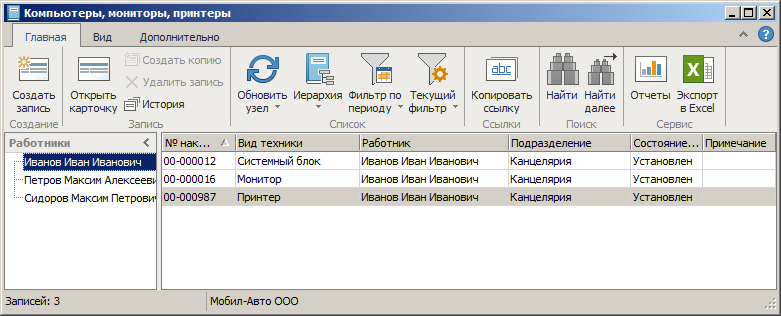
\includegraphics[width=\textwidth]{pic9.png}}
\end{frame}
\lecturenotes
С помощью использования иерархии по работникам организации отображается список техники закреплённой за определенным сотрудником.

\begin{frame} \frametitle{Достоинства DIRECTUM}
Достоинства Helpdesk на базе DIRECTUM:
	\begin{itemize}
		\item работа всех сотрудников организации в едином информационном пространстве
		\item адаптируемость к нуждам организации с помощью инструментов разработки DIRECTUM
		\item поддержка одной системы DIRECTUM вместо поддержки нескольких систем: других программ типа Help Desk и/или учета техники
		\item статистика обращений по количеству и типу заявок
		\item заявки не теряются и находятся под контролем сотрудников и начальника службы поддержки
		\item возможность приложить к заявке ссылки на объекты DIRECTUM (документы или записи справочников)
		\item простота использования
	\end{itemize}
\end{frame}
\lecturenotes

\subsection{Итилиум}
\begin{frame} \frametitle{1С Итилиум}

    Итилиум -- это российский Service Desk для автоматизации службы обработки заявок и процессов управления IT, изначально разрабатывался как массовая система. Его применяют с платформами «1С:Предприятие» 8.2 и 8.3

\end{frame}
\lecturenotes

\begin{frame} \frametitle{Интерфейс}
\centerline{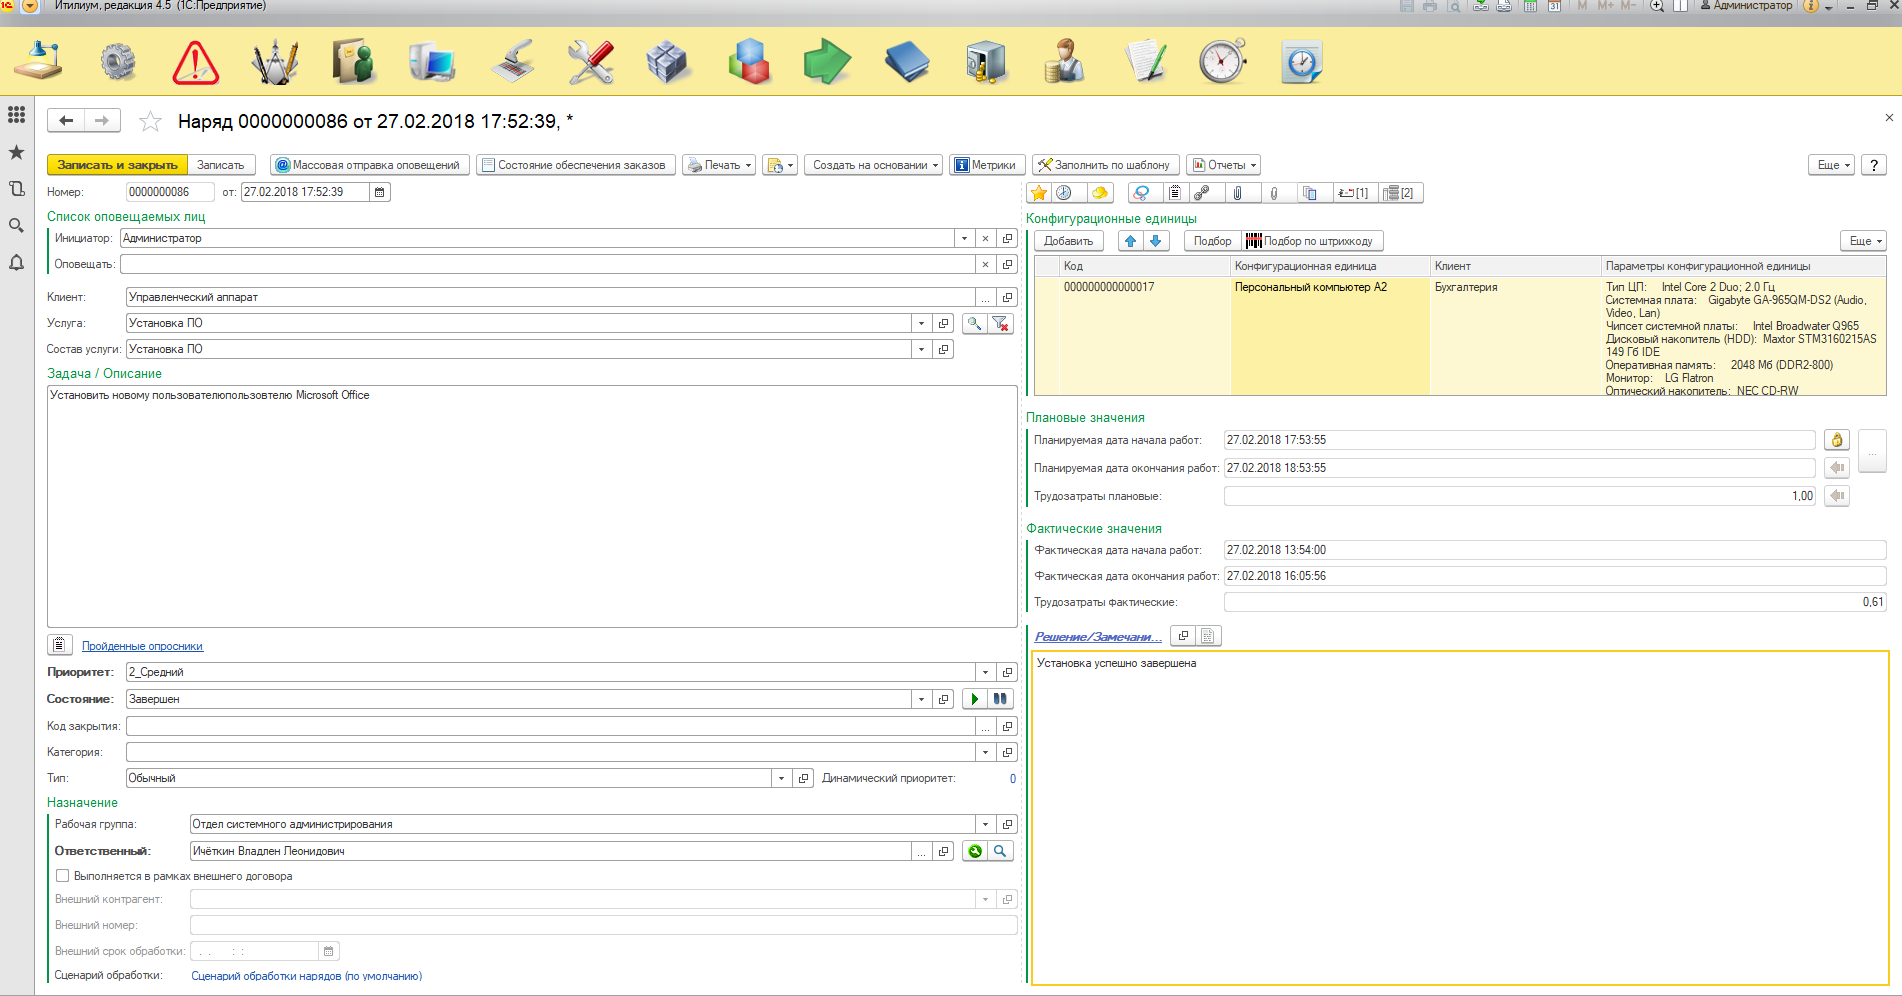
\includegraphics[width=\textwidth]{pic10.png}}
\end{frame}
\lecturenotes


\begin{frame} \frametitle{Основные возможности}
	\begin{itemize}
    \item Управление уровнем услуг
    \item Управление инцидентами
    \item Управление запросами на обслуживание
    \item Управление проблемами
    \item Управление изменениями
    \item Управление работами
    \item Управление конфигурациями и активами
    \item Управление релизами
	\end{itemize}
\end{frame}
\lecturenotes

\begin{frame} \frametitle{Пример обращения}
\centerline{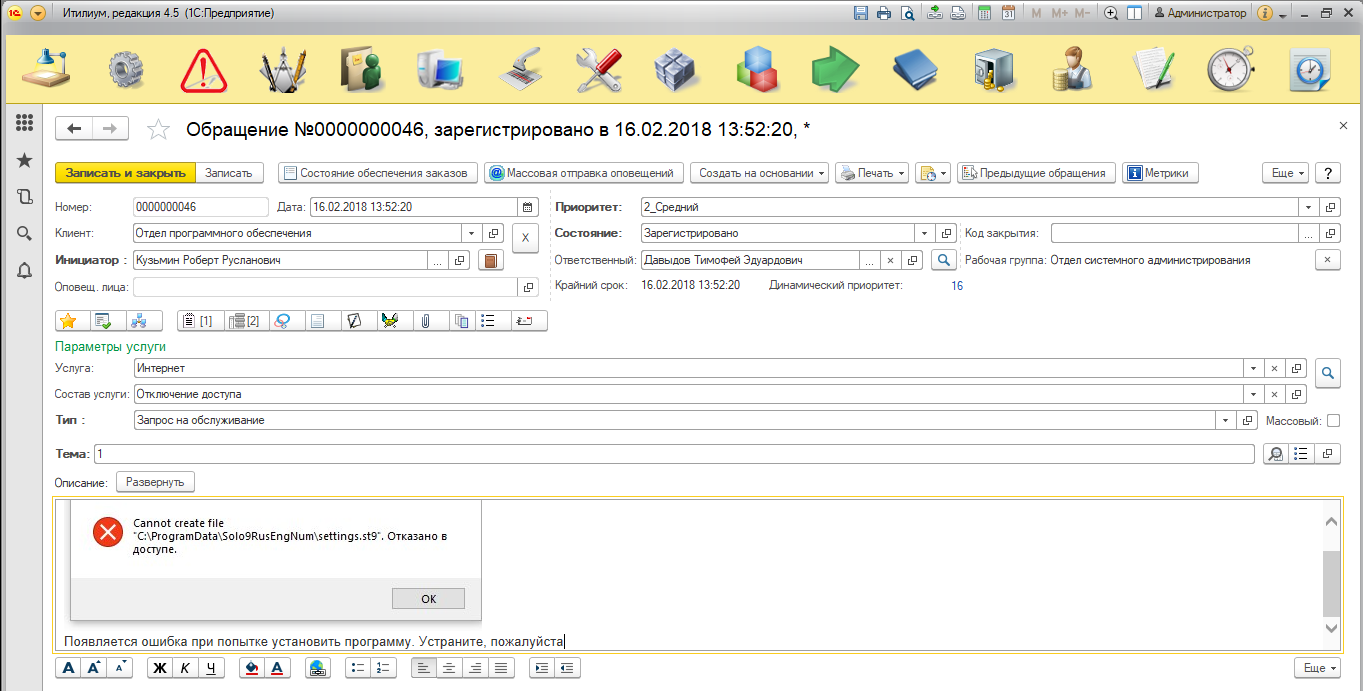
\includegraphics[width=\textwidth]{pic12.png}}
\end{frame}
\lecturenotes

\begin{frame} \frametitle{Возможности управления инцидентами}
	\begin{itemize}
    \item Регистрация инцидентов, контроль сроков решения инцидентов
    \item Поддержка схем эскалаций (передача ответственности, уведомления)
    \item Управление нарядами
    \item Поддержка базы знаний по решению инцидентов
	\end{itemize}
\end{frame}
\lecturenotes

\begin{frame} \frametitle{Возможности управления проблемами}
	\begin{itemize}
    \item Выявление и регистрация проблем
    \item Ведение перечня «известных ошибок»
    \item Управление конфигурациями и изменениями
    \item Учет конфигурационных элементов и изменений
    \item Связь с инцидентами, проблемами, нарядами
    \item Хранение документооборота по ИТ активам (конфигурационным элементам), изменениям
	\end{itemize}
\end{frame}
\lecturenotes

\begin{frame} \frametitle{Динамика обращений}
\centerline{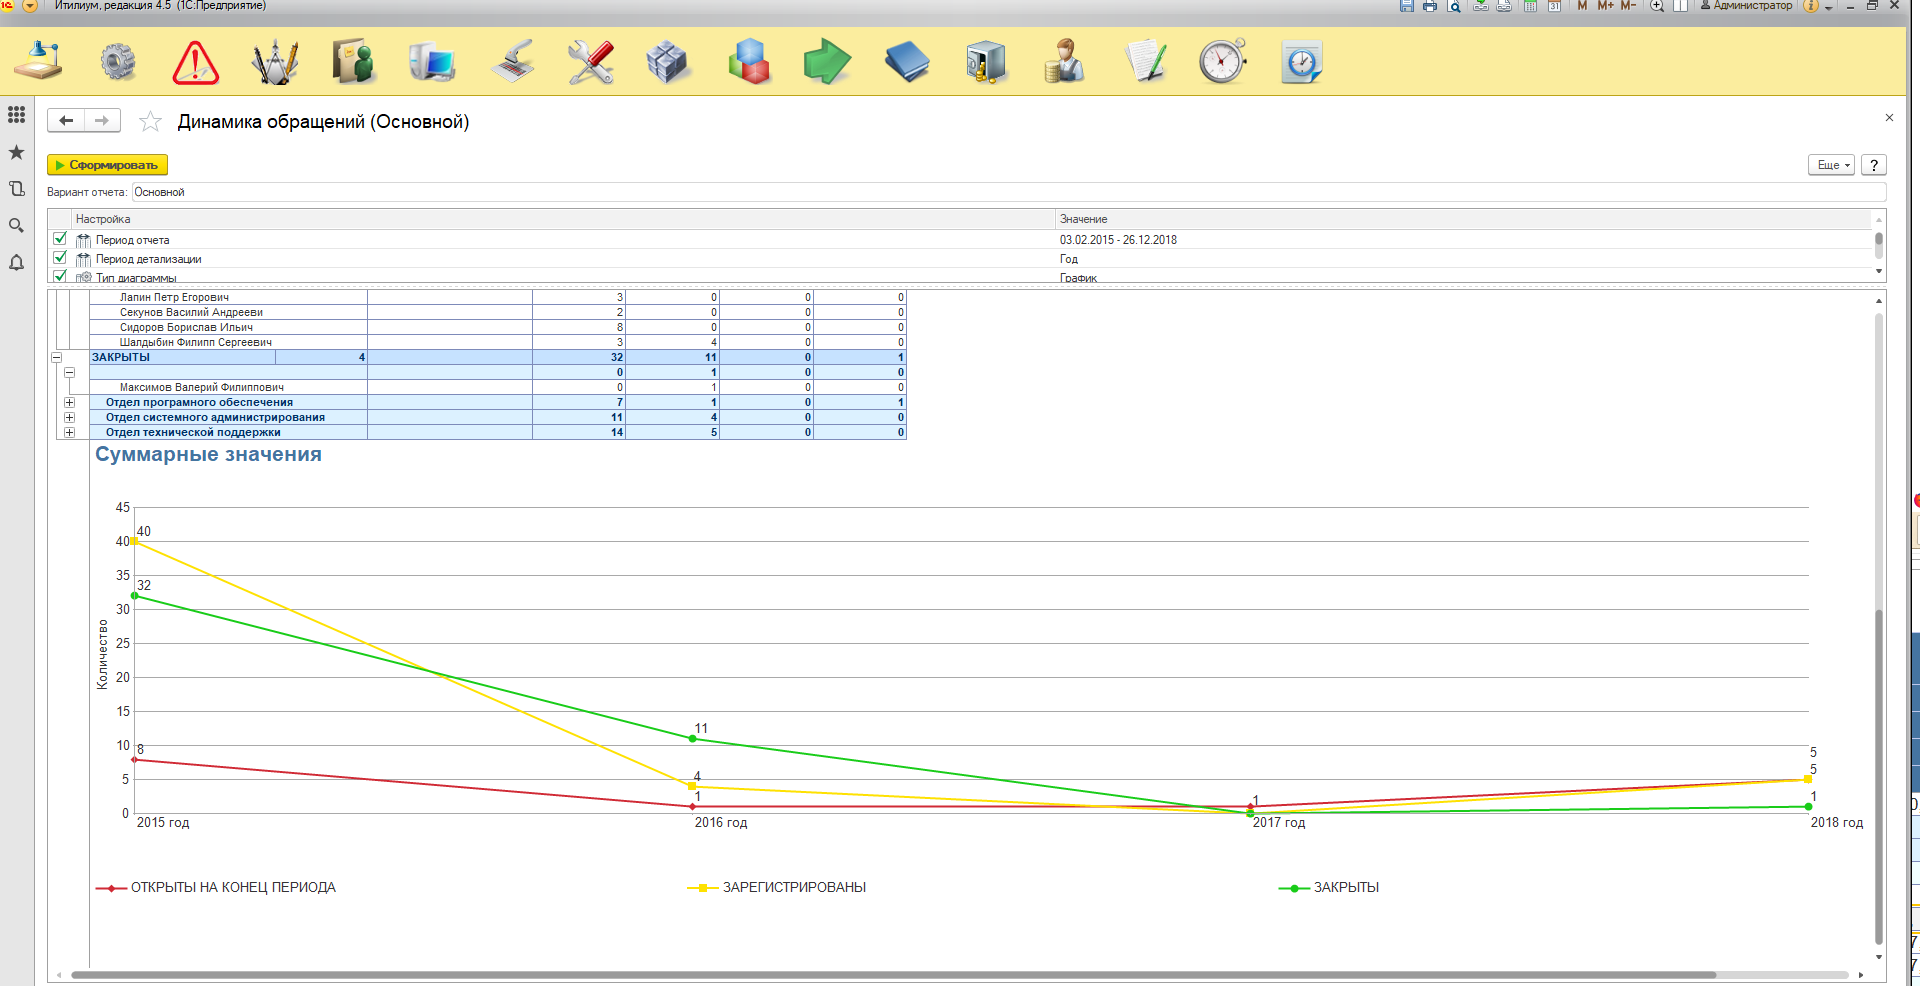
\includegraphics[width=\textwidth]{pic11.png}}
\end{frame}
\lecturenotes

\begin{frame} \frametitle{Реестр обращений}
\centerline{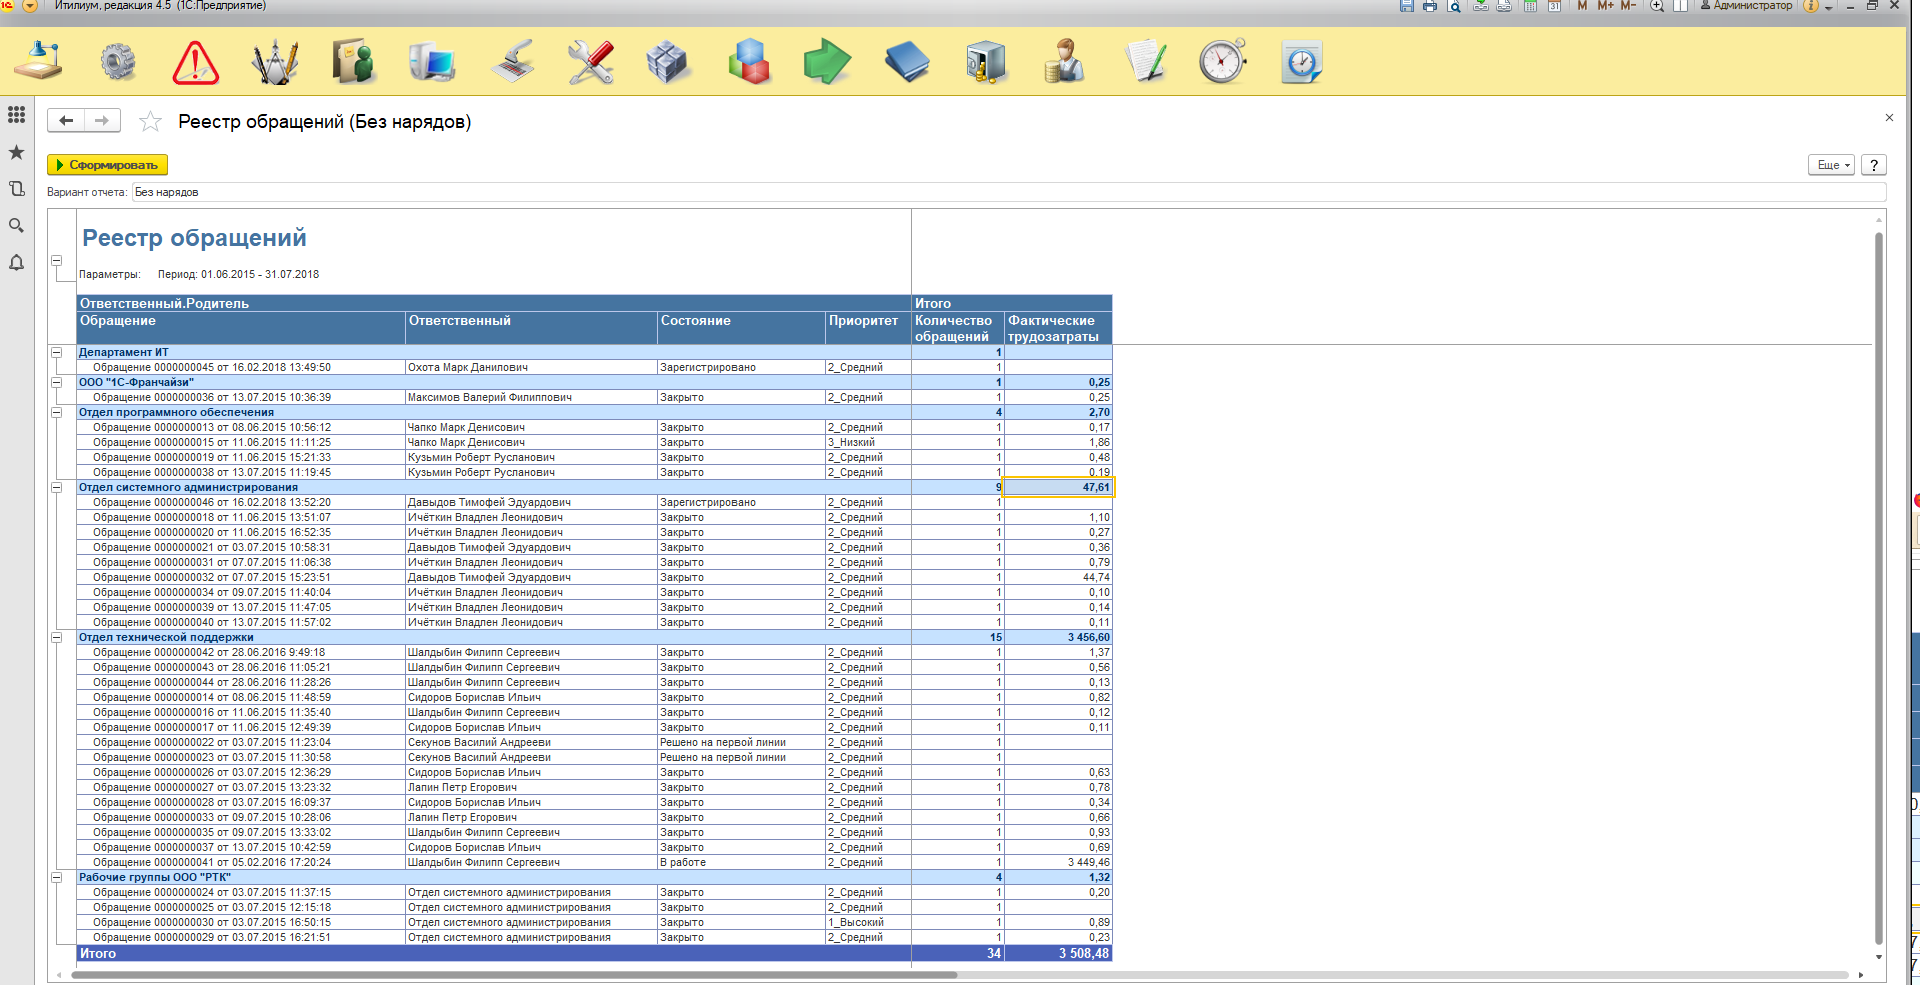
\includegraphics[width=\textwidth]{pic14.png}}
\end{frame}
\lecturenotes

\begin{frame} \frametitle{Отчет по качеству выполнения обращений}
\centerline{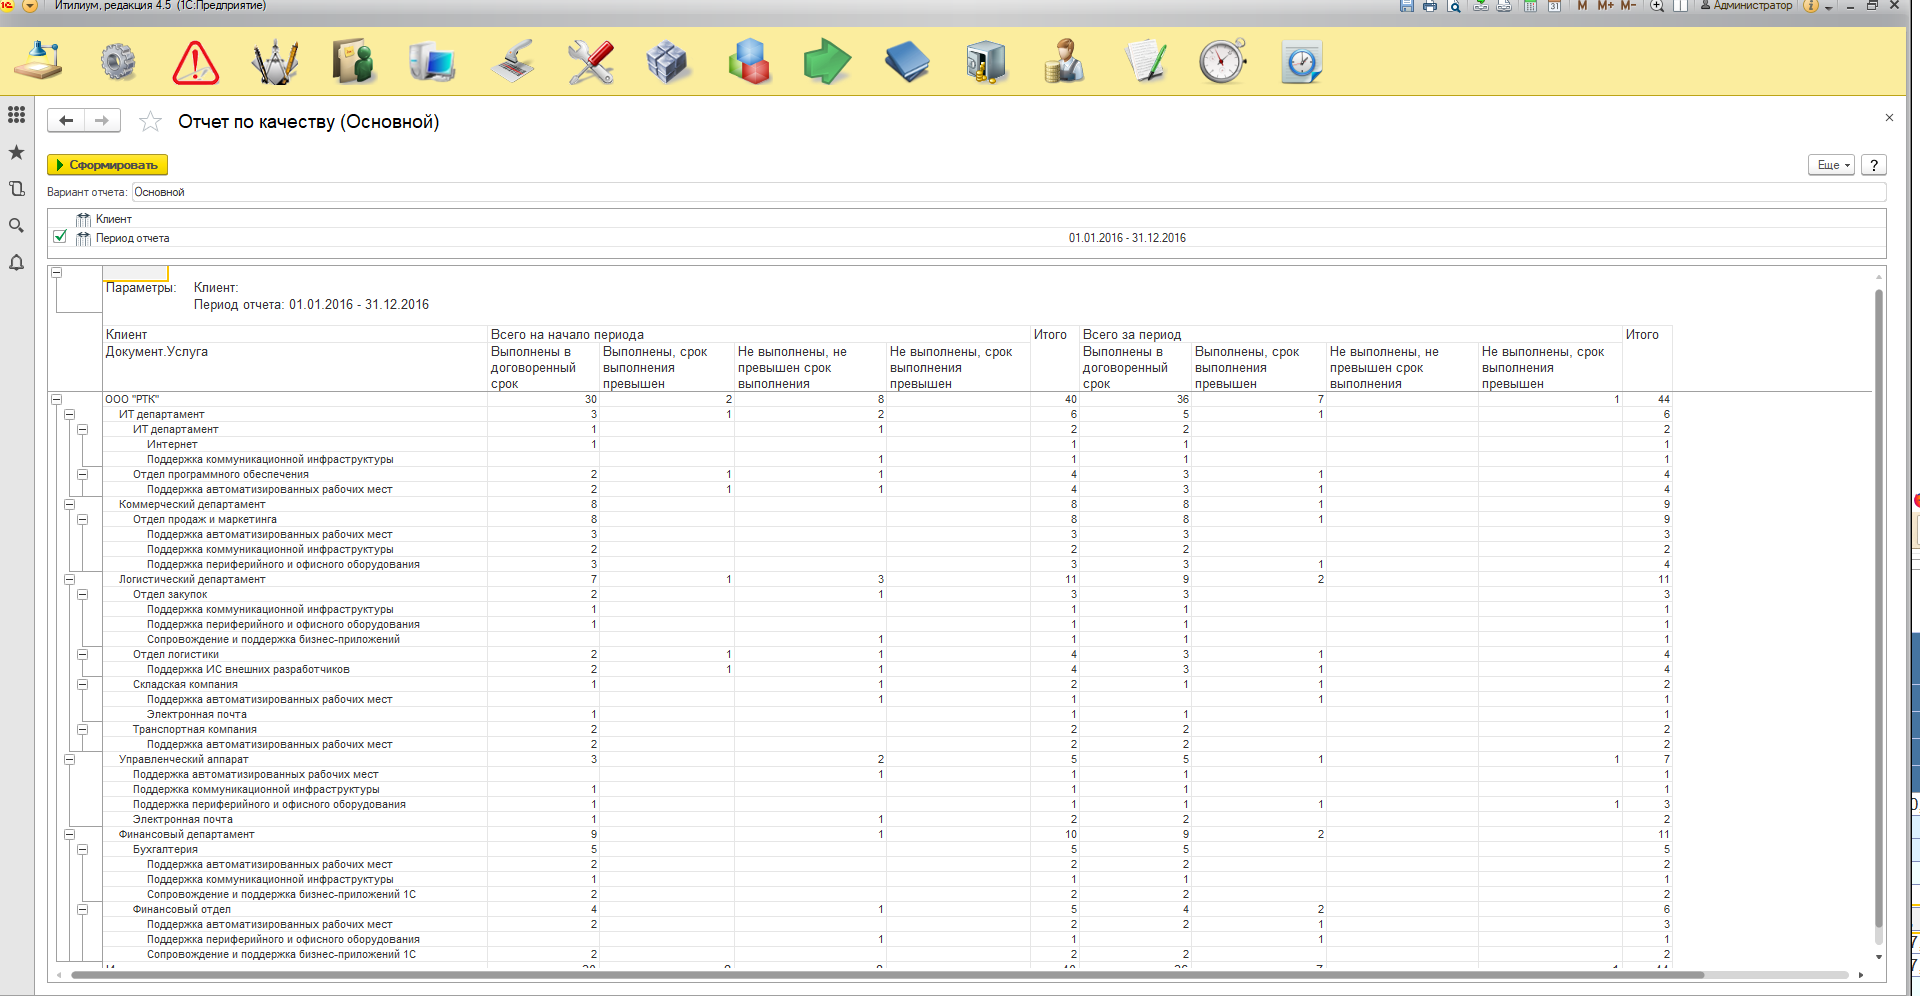
\includegraphics[width=\textwidth]{pic13.png}}
\end{frame}
\lecturenotes

\begin{frame} \frametitle{Достоинства Итилиум}
	\begin{itemize}
		\item Широкий функционал
		\item Гибкость системы благодаря открытому коду
		\item Методика внедрения, методические материалы, обучающие семинары входят в стоимость внедрения
		\item Самостоятельное внедрение или полная настройка специалистами 
		\item Система метрик и показателей, позволяющая строить статистику
		\item Совместимость с 1С, логика и интерфейс знакомы 1С-специалистам
		\item Методологическая русскоязычная поддержка
		\item Возможность использования мобильных устройств
	\end{itemize}
\end{frame}
\lecturenotes


\end{document}

%%% Local Variables: 
%%% mode: TeX-pdf
%%% TeX-master: t
%%% End: 
